\section{Critical Analysis}
\label{sec:critical_analysis}

\subsection*{(a) When does R-SGD help?}

In the tasks described above, R-SGD did not demonstrate any performance gain 
over standard SGD. This outcome is consistent with our experimental setup. 
We introduced additive isotropic Gaussian noise, meaning the observed gradient 
covariance is
\begin{equation}
    \operatorname{Cov}(v_i) = \operatorname{Cov}(u_i) + \sigma^2 I .
\end{equation}
If the added noise dominates the variation of the clean gradients, the estimated 
uncertainty matrix $S_k$ becomes approximately isotropic, $S_k \approx s I$. Under 
this condition, as derived in Section~\ref{sec:isotropic_noise}, the optimal robust 
step simplifies to:
\begin{equation}
    d_k = -\alpha_k \left( 1 - \frac{\rho \sqrt{s}}{|g_k|} \right)_+ g_k .
    \label{eq:robust_step_isotropic}
\end{equation}
This equation shows that for isotropic uncertainty, the robust step $d_k$ is collinear with the negative batch gradient $-g_k$. R-SGD does not change the update direction; it merely scales the step length. Because R-SGD and SGD take different step lengths, they do not follow the exact same trajectory; their subsequent states diverge, leading to different gradients at the next iteration. Nevertheless, since both update in the same direction at any given state, R-SGD provides no directional advantage. It effectively acts as a step-size regularizer, a role that can be fulfilled by tuning the learning rate of standard SGD. Therefore, in our setup, R-SGD introduces unnecessary computational overhead.

R-SGD is theoretically positioned to help when the noise is strongly anisotropic or when the clean gradient covariance has vastly different directional scales, forcing the optimizer to rotate its step away from heavily corrupted directions. However, testing such structured anisotropic noise was outside the scope of this work.

\subsection*{(b) Interactions among radius, covariance, and learning rate}

The tuning heatmap (Figure \ref{fig:sim1_tuning}) illustrates the interaction between these three parameters. 
First, at sub-optimal learning rates (e.g., \(lr = 0.01\) or \(0.1\)), increasing the radius \(\rho\) slightly improves validation loss. Here, robustness acts as a form of regularization, preventing the optimizer from taking overly aggressive, unstable steps in noisy directions. However, at the optimal learning rate (\(lr = 1.0\)), the loss remains mostly flat across small radii and then degrades for large \(\rho\).

This degradation is directly linked to the zero steps before reaching a minimizer. As the radius \(\rho\) increases, the uncertainty ball expands. When the condition \(g_k^T S_k^{-1} g_k \le \rho^2\) is met, the robust step \(d_k\) is set to exactly zero. If \(\rho\) is too large relative to the covariance \(S_k\), the optimizer essentially "freezes" prematurely, halting its progress long before reaching the true minimum. The covariance \(S_k\) determines the shape of this uncertainty ball, while the learning rate dictates the baseline step size; if \(\rho\) is large enough to trigger zero-steps frequently, the learning rate becomes irrelevant because the updates are suppressed.


\begin{figure}[htbp]
    \centering
    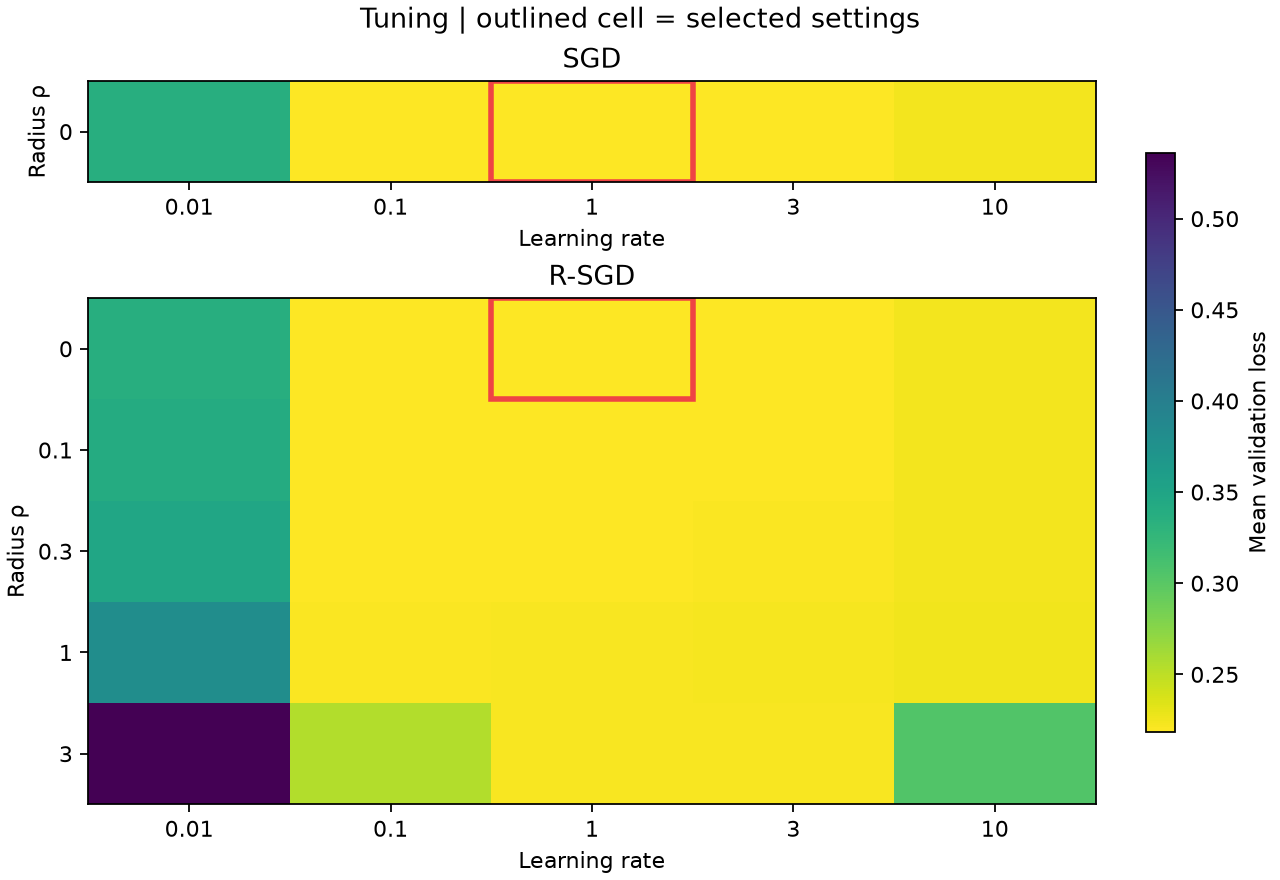
\includegraphics[width=0.8\textwidth]{./plots/logreg/tuning.png}
    \caption{Interactions among radius, covariance, and learning rate.}
    \label{fig:sim1_tuning}
\end{figure}

\subsection*{(c) Does lower training loss imply higher test accuracy?}

No, lower training loss does not necessarily imply higher test accuracy, and our 
experiments clearly demonstrate this divergence. In both simulations, we observed 
noticeable variations in training and validation loss (especially when testing different radii), 
yet the test accuracy remained almost perfectly stable.

This discrepancy arises from the fundamental difference between the two metrics. Loss is a 
continuous measure: it penalizes the model based on the confidence of its predictions. 
A minor shift in the decision boundary will immediately change the loss. 
Accuracy, on the other hand, is a discrete metric: it only evaluates whether a prediction 
crosses the classification threshold. The decision boundary can shift, 
changing the loss, but as long as no data points cross that boundary, the accuracy remains 
strictly identical. Thus, optimization quality (loss) and predictive performance (accuracy) are distinct outcomes.

\subsection*{(d) Limitations and Future Work}

\textbf{Limitation 1: Isotropic noise only.} The primary limitation of our study is the exclusive use of isotropic noise. As shown in part (a), this fails to leverage the directional filtering capabilities of R-SGD. 
\textit{Focused next experiment:} Introduce anisotropic noise. \textit{Hypothesis:} R-SGD will significantly outperform SGD here, as the covariance matrix \(S_k\) will correctly identify the noisy dimensions and rotate the step away from them.

\textbf{Limitation 2: Fixed batch size.} We kept the batch size constant across all runs. However, the batch size directly dictates the variance of the covariance estimate \(S_k\). With a small batch, \(S_k\) is highly noisy; with a large batch, it is accurate but computationally expensive.
\textit{Focused next experiment:} Sweep the batch size under a fixed high noise level. 
\textit{Hypothesis:} With a very small batch size, R-SGD will underperform due to the noisy 
estimation of \(S_k\). As the batch size increases, the estimate \(S_k\) stabilizes, and the 
performance of R-SGD should improve, potentially matching or slightly exceeding SGD's stability 
before the computational overhead becomes prohibitive.